% Flow-only variant of fig_methodflow (block diagram; the substrate half is the teaser).
% parallel to an illustration of what each layer sets on the substrate
% (right): tiles mapped onto the 3D mesh, and a zoom into one node showing
% the port loads (PIL/PEL -> PF, packing-fixed) and the link load
% (Lambda_l -> PL, placement-set).  Concepts only: no result numbers.
% Standalone; pdflatex fig_methodflow.tex -> fig_methodflow.pdf
\documentclass[border=3pt]{standalone}
\usepackage{times}
\usepackage{amsmath}
\usepackage{tikz}
\usetikzlibrary{arrows.meta,positioning,calc,fit,backgrounds}

\definecolor{cPack}{HTML}{2A78D6}   % packing
\definecolor{cMap}{HTML}{EB6834}    % mapping / PL
\definecolor{cRoute}{HTML}{1BAF7A}  % routing
\definecolor{cInk}{HTML}{101720}
\definecolor{cInk2}{HTML}{3A4653}
\definecolor{cFaint}{HTML}{9AA5B1}
\definecolor{cGridL}{HTML}{C9D2DB}

\begin{document}
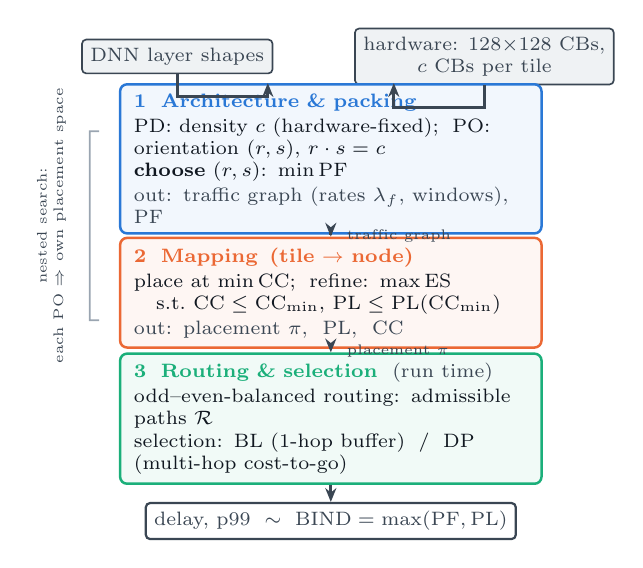
\begin{tikzpicture}[
  font=\scriptsize,
  ar/.style={-{Stealth[length=4.5pt,width=3.5pt]},line width=0.8pt,color=cInk2},
  flow/.style={-{Stealth[length=5pt,width=4pt]},line width=1.0pt,color=cInk2},
  lead/.style={line width=0.5pt,color=cFaint,densely dashed},
  lbl/.style={font=\scriptsize,color=cInk,align=center},
  sub/.style={font=\tiny,color=cInk2,align=center},
  blk/.style={draw,rounded corners=2.5pt,line width=0.9pt,align=left,
              inner xsep=5pt,inner ysep=3.5pt,text width=50mm,font=\scriptsize},
  io/.style={draw,line width=0.6pt,color=cInk2,fill=cGridL!30,rounded corners=1.5pt,
             align=center,inner sep=3pt,font=\scriptsize},
  tag/.style={font=\tiny\bfseries,text=white,inner sep=2pt,rounded corners=1pt},
]

% ====================================================== LEFT: the design flow
% inputs
\node[io] (inDNN) at (0.0,5.35) {DNN layer shapes};
\node[io] (inHW)  at (3.9,5.35) {hardware: $128{\times}128$ CBs,\\$c$ CBs per tile};

% -- layer 1: architecture & packing
\node[blk,color=cPack,fill=cPack!6,text=cInk] (L1) at (1.95,4.05)
  {\textbf{\textcolor{cPack}{1\; Architecture \& packing}}\\[1pt]
   PD: density $c$ (hardware-fixed);\; PO: orientation $(r,s)$, $r\cdot s=c$\\
   \textbf{choose} $(r,s)$: $\min \mathrm{PF}$\\[1pt]
   \textcolor{cInk2}{out: traffic graph (rates $\lambda_f$, windows),\ \ $\mathrm{PF}$}};

% -- layer 2: mapping
\node[blk,color=cMap,fill=cMap!6,text=cInk] (L2) at (1.95,2.35)
  {\textbf{\textcolor{cMap}{2\; Mapping \,(tile $\to$ node)}}\\[1pt]
   place at $\min \mathrm{CC}$;\; refine: $\max \mathrm{ES}$\\
   \quad s.t.\ $\mathrm{CC}\le\mathrm{CC}_{\min}$, $\mathrm{PL}\le\mathrm{PL}(\mathrm{CC}_{\min})$\\[1pt]
   \textcolor{cInk2}{out: placement $\pi$,\ \ $\mathrm{PL}$,\ \ $\mathrm{CC}$}};

% -- layer 3: routing & selection
\node[blk,color=cRoute,fill=cRoute!6,text=cInk] (L3) at (1.95,0.75)
  {\textbf{\textcolor{cRoute}{3\; Routing \& selection}}\ \ \textcolor{cInk2}{(run time)}\\[1pt]
   odd--even-balanced routing: admissible paths $\mathcal R$\\
   selection: BL (1-hop buffer)\; /\; DP (multi-hop cost-to-go)};

% -- output
\node[io,fill=white,line width=0.8pt] (out) at (1.95,-0.55)
  {delay, p99 \;$\sim$\; $\mathrm{BIND}=\max(\mathrm{PF},\mathrm{PL})$};

% flow arrows
\draw[flow] (inDNN.south) -- ++(0,-0.28) -| ($(L1.north)+(-0.8,0)$);
\draw[flow] (inHW.south)  -- ++(0,-0.28) -| ($(L1.north)+(0.8,0)$);
\draw[flow] (L1.south) -- (L2.north) node[midway,right=2pt,sub]{traffic graph};
\draw[flow] (L2.south) -- (L3.north) node[midway,right=2pt,sub]{placement $\pi$};
\draw[flow] (L3.south) -- (out.north);

% nested search bracket
\draw[line width=0.6pt,color=cFaint] ($(L1.west)+(-0.25,0.35)$) -- ++(-0.12,0)
   -- ($(L2.west)+(-0.37,-0.35)$) -- ++(0.12,0);
\node[sub,rotate=90,anchor=south,color=cInk2] at ($(L1.west)!0.5!(L2.west)+(-0.55,0)$)
   {nested search:\\each PO $\Rightarrow$ own placement space};

\end{tikzpicture}
\end{document}
